\documentclass{report}
\usepackage[a4paper, portrait, top=20mm, left=20mm, right=20mm, bottom=20mm]{geometry}
\usepackage{graphicx,wrapfig,amsmath,amssymb,xcolor,pgfplots,adjustbox,float,tikz}
\usepackage[colorlinks=true,urlcolor=blue,labelcolor=black]{hyperref}
\usepackage[utf8]{inputenc}

\newcommand{\tr}[1]{{{#1}^\top}} % transpose
\newcommand{\w}{\mathbf{w}} % vectors
\newcommand{\x}{\mathbf{x}}
\newcommand{\y}{\mathbf{y}}

\DeclareMathOperator*{\argmax}{arg\,max}
\DeclareMathOperator*{\argmin}{arg\,min}

\newcommand{\loss}{\mathcal{L}}

\setlength{\parindent}{0pt}

\title{Artificial Intelligence and Machine Learning}
\author{Abhijit Amrendra Kumar}
\date{August 2023}

\begin{document}

\maketitle

\chapter{Introduction}
\section{What is Machine Learning ?}

Machine learning is the ability of machines to \textbf{learn} from data or past experiences, which come from various sources such as sensors, domain knowledge, experimental runs, etc. Mathematically, it involves making a theoretical function/model $f: X \rightarrow Y$ which predicts outcomes from given inputs, and optimizing it and training it to increase it's prediction accuracy.

\section{Why Machine Learning ?}

We need machine learning in the following cases
\begin{itemize}
  \item When we need to perform tasks that are easy for humans, but complex for computer systems to emulate (eg. distinguishing between a muffin and a Chihuahua)
  \item When we need to perform tasks which are beyond human capabilities, like the analysis of large and complex datasets
\end{itemize}

\begin{center}
  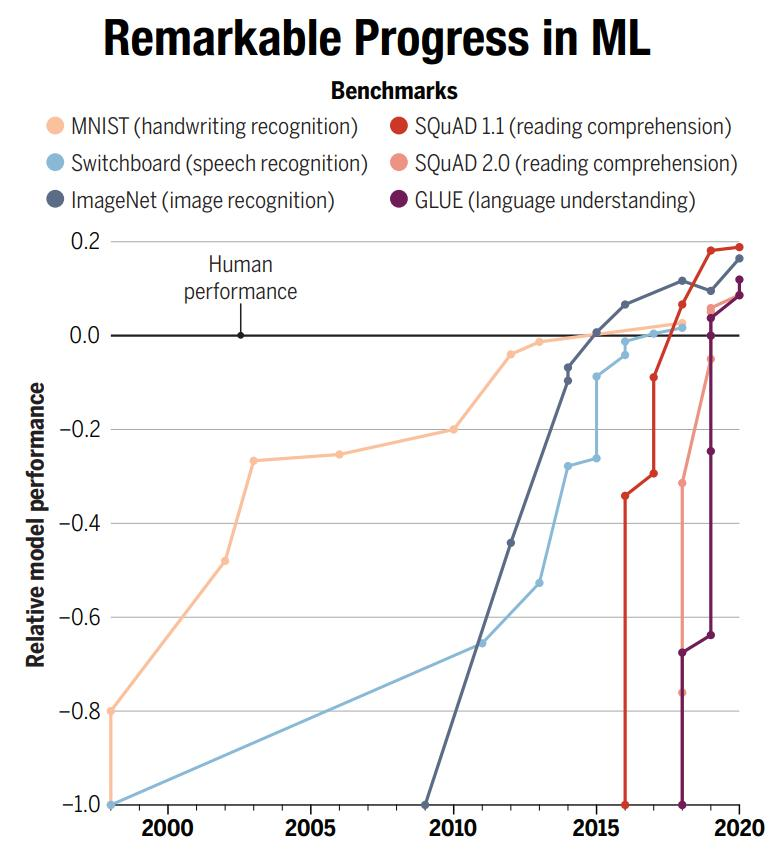
\includegraphics[scale=0.25]{"images/aiml-01.jpg"}
\end{center}

Here is a usage histogram for various ML algorithms, which indicates that linear regression and decision trees are very likely to be useful in a machine learning problem.

\begin{center}
  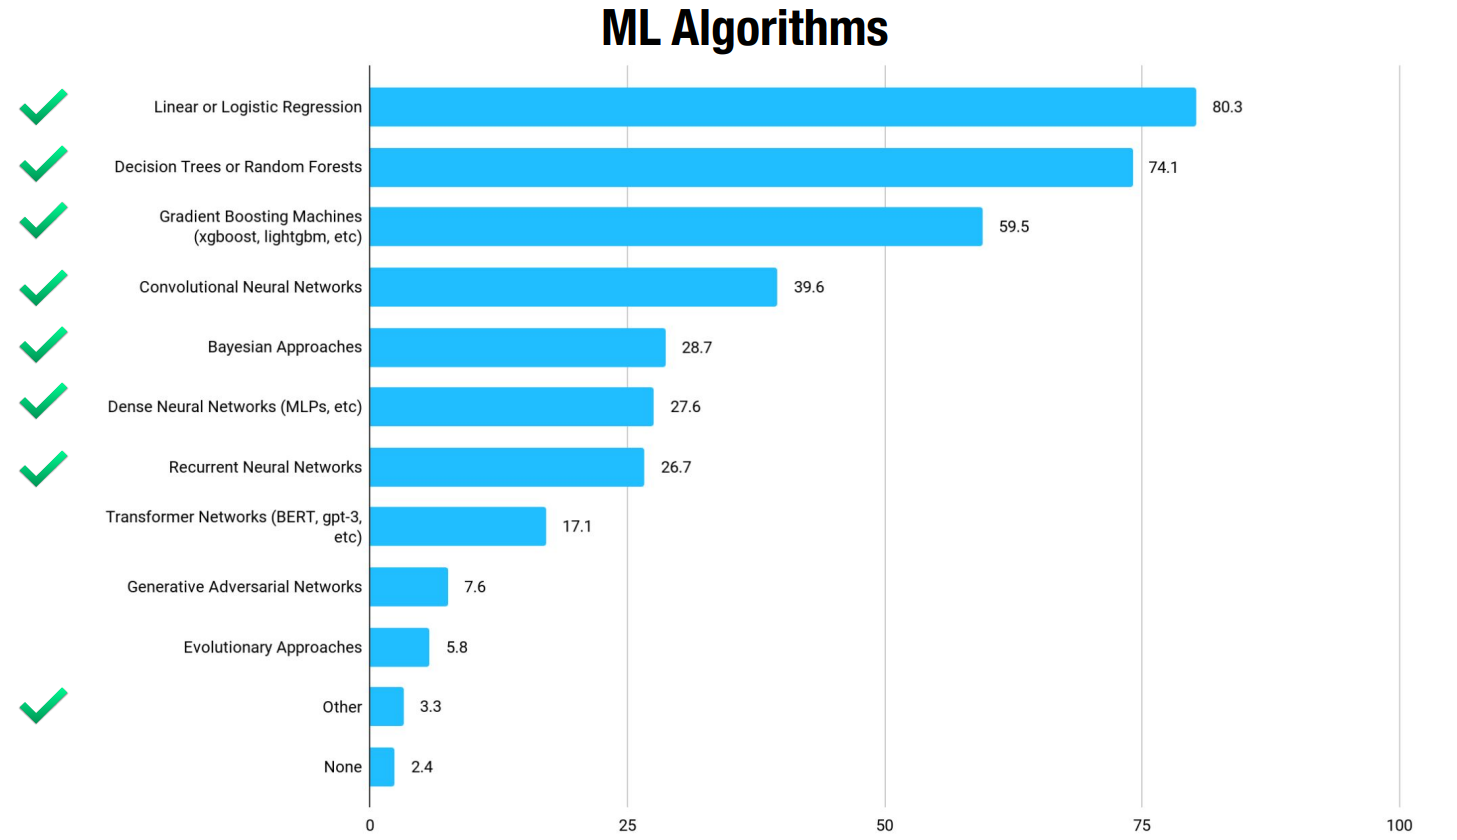
\includegraphics[scale=0.2]{"images/aiml-02.png"}
\end{center}

\section{ML Pipeline}
\begin{itemize}
  \item \textbf{Data}: Collect data for your problem
        \begin{itemize}
          \item Is the data labelled or unlabelled ?
        \end{itemize}
  \item \textbf{Representation}: Choose features that represent your data
        \begin{itemize}
          \item Is the data representation raw, expert-derived or learned ?
        \end{itemize}
  \item \textbf{Modeling}: Choose a model for a task
        \begin{itemize}
          \item Should the model be linear/non-linear ? Also, what will be the computational overheads ?
        \end{itemize}
  \item \textbf{Training/Learning}: Model will (likely) be parameterized, and these parameters will be learned by training over the data. So, choose a loss function to optimize.
        \begin{itemize}
          \item Which loss function to choose ? And how to best optimise this loss function ?
        \end{itemize}
  \item \textbf{Prediction/Inference}: Given a model, assign labels to unseen test instances, then choose an evaluation metric.
        \begin{itemize}
          \item Is the evaluation manual or automatic ?
        \end{itemize}
\end{itemize}

\section{Resources}
Here are some links to find various datasets
\begin{itemize}
  \item \href{https://archive.ics.uci.edu/}{https://archive.ics.uci.edu/}
  \item \href{https://huggingface.co/datasets}{https://huggingface.co/datasets}
  \item \href{http://www.openslr.org/}{http://www.openslr.org/}
\end{itemize}

% ----------------------------------------------------------------

\chapter{Linear Regression}

\section{Notation}

In general we format variables as: $x$ for scalars, $\x$ for vectors, and $X$ for matrices.
\begin{itemize}
  \item Input / Feature space / Attributes Space :  \( \mathcal{X} =  \mathbb{R}^d\) for some \(d\in\mathbb{N}\)
  \item Output / \emph{Label space} / Response space : \( \mathcal{Y}= \mathbb{R} \)
  \item Dataset : \( \mathcal{D} = \left\{(\textbf{x}_i,y_i)\right\}_{i=1}^{n} \), where \(\textbf{x}_i \in \mathcal{X}, y_i \in \mathcal{Y} \ \forall \ i \in \{1\ldots n\}\)
\end{itemize}

We consider a target function $f : \mathcal{X} \to \mathcal{Y}$ on the training dataset $\mathcal{D}$, i.e. $\textbf{x} \overset{f}{\mapsto} y \ \forall \ (\x,y) \in \mathcal{D}$. \\

We focus on the task of finding a \emph{hypothesis function} \(h : \mathcal{X} \to \mathcal{Y}\) that ideally closely approximates \(f\). We call the family of the hypothesis functions as \(\mathcal{H}\), the \emph{Hypothesis Class}. It follows that \(h \in \mathcal{H}\)
This now brings the following questions:
\begin{enumerate}
  \item What are the possibilities for the predictor function \(h\) ? [\textbf{Hypothesis Class}]
  \item How do you quantify the performance of the predictor? [\textbf{Loss/Error Function}]
  \item How do we find the best predictor? [\textbf{Optimization}]
\end{enumerate}

\section{What are the possible predictor functions?}

Let us first play with a simpler case with a one-dimensional feature space. We may consider the problem as a line fitting problem, taking our hypothesis class to be all linear functions.

\begin{figure}[H]
  \centering
  \begin{tikzpicture}
    \begin{axis}[
        axis lines=middle,
        xlabel=$x$,
        ylabel=$y$,
        xmin=0, xmax=10,
        ymin=0, ymax=15,
        xtick={0,2,...,5},
        ytick={0,3,...,9},
        grid=both,
        grid style={line width=0.1pt, draw=gray!30},
      ]
      \addplot[only marks, mark=*, blue] coordinates {
          (1, 2)
          (2, 4)
          (3, 5)
          (4, 7)
          (5, 8)
          (2,9)
          (4,2)
          % Add more data points here
        };
      \addplot[red] {1.5*x + 0.5}; % Change the slope and intercept as needed
    \end{axis}
  \end{tikzpicture}
  \caption{Fitting a line to the data}
\end{figure}

Let us parametrize the line with $w_0,w_1$ (intercept and slope). We can vectorize our parameters as $W = \begin{bmatrix} w_0 \\ w_1 \end{bmatrix}$. Then we may write our hypothesis function $h_\w$ parametrised by $\w$ as.

$$
  h_\w(x) = w_0 + w_1 x
$$

Let us also vectorize our input as $\x = \begin{bmatrix} 1 \\ x \end{bmatrix}$, so that
$$
  h_{\w}(\x) = \tr{\w} \x
$$

We can now extend this to the multidimensional case. We consider our function to return a linear combination of our \(d\) dimensional features. \newline

\begin{figure} [h]
  \centering
  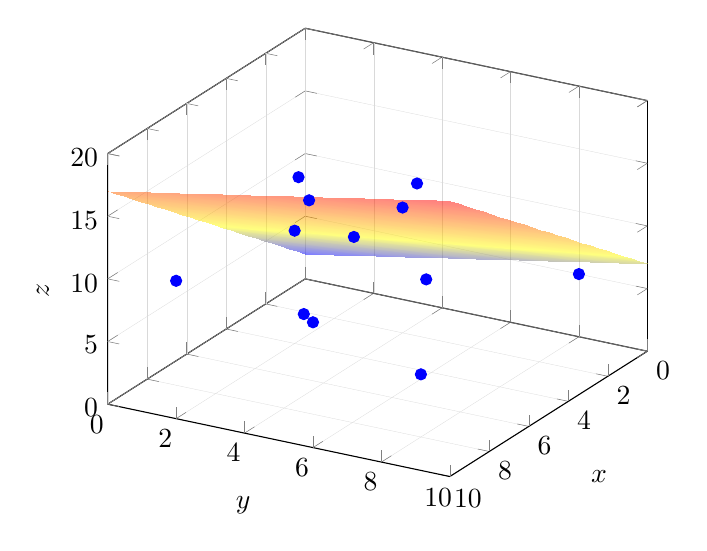
\begin{tikzpicture}
    \begin{axis}[
        view={120}{30},
        xlabel=$x$,
        ylabel=$y$,
        zlabel=$z$,
        xmin=0, xmax=10,
        ymin=0, ymax=10,
        zmin=0, zmax=20,
        xtick={0,2,...,10},
        ytick={0,2,...,10},
        ztick={0,5,...,20},
        grid=both,
        grid style={line width=0.1pt, draw=gray!30},
      ]

      \addplot3[only marks, mark=*, blue] coordinates {
          (0,8,5)
          (1, 2, 5.5)
          (2, 4, 10)
          (3, 5, 13.5)
          (4, 2, 9)
          (5, 3, 13)
          (6, 7, 10)
          (7, 4, 6.5)
          (8, 8, 5)
          (9, 5, 20)
          (10, 6, 10)
          (10, 2, 11)
        };

      \addplot3[
        surf,
        opacity=0.5,
        shader=interp,
        domain=0:10,
        domain y=0:10,
      ] {1.5*x + 0.5*y + 2}; % Adjust the coefficients as needed

    \end{axis}
  \end{tikzpicture}
  \caption{For higher dimensional feature spaces, linear regression is akin to \emph{Hyperplane Fitting}}
\end{figure}

We now have our parameter \(\w = \begin{bmatrix}w_0\\w_1\\\vdots\\w_d\end{bmatrix} \in \mathbb{R}^{d+1}\) and input vector \(\x = \begin{bmatrix}1\\x_1\\\vdots\\x_d\end{bmatrix}\) to get a identical expression -

$$
  h_\w(\x) = \tr{\w} \x
$$
Our hypothesis class is, then -
$$
  \mathcal{H} = \{ h_\w : \w \in \mathbb{R}^{d+1} \}
$$

This is essentially the \textit{linear} in linear regression. However, note that it does not mean we are restricted to linear functions of the features, we may transform the feature space to another space to regress.

\section{How to quantify the performance of a predictor ?}

We define a function that operates on the predictor function and dataset to quantify the "mismatch" between the two. Higher the loss function, lesser is the given predictor suitable for the dataset. Given that our function is parametrized, we may also define the loss function in terms of the parameter.

$$
  \text{Loss Function: } \loss(h,\mathcal{D}) ~\text{or}~ \loss(\w,\mathcal{D})
$$

Let us consider a singleton dataset $\mathcal{D}_{test} =\{(\x,y)\}$ where $\x = \tr{\left[1~x_1~\ldots~x_d\right]}$. We define a loss for this dataset as
$$
  \loss(\w,\mathcal{D}_{test}) = (y-h_\w(\x))^2 = |y-\hat{y}|^2
$$

We define \(h_\w(x) = \hat{y}\), and \(|y-\hat{y}|\) is called a \emph{residual}. \\

Now for a dataset containing $n$ datapoints,

$$
  \mathbf{Least\ Squares\ Loss:} \ \  \loss(\w,\mathcal{D}_{train}) = \frac{1}{n} \sum_{i=1}^n(y_i-h_\w(\x_i))^2 = \frac{1}{n} \sum_{i=1}^n \left|y_i - \hat{y}_i\right|^2
$$

Note that the least squares loss is the mean of the squares of the residuals. We can also define a loss equal to the mean residual value.

$$
  \text{Mean Absolute Error Loss:} \ \ \loss({\w,\mathcal{D}_{train}}) = \frac{1}{n} \sum_{i=1}^n \left|y_i - \hat{y}_i\right|
$$

The Mean Absolute Error does not penalise high deviations as much as the Squares Loss, thus it may be more appropriate to use when the dataset contains many outliers.
\begin{figure}[htbp]
  \centering
  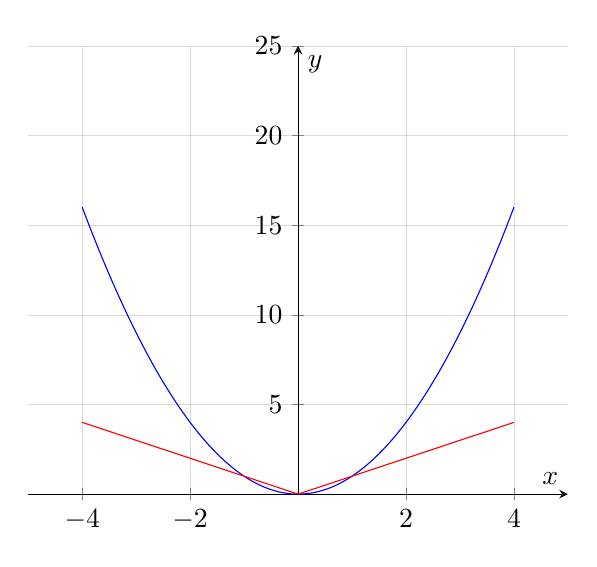
\begin{tikzpicture}
    \begin{axis}[
        axis lines=middle,
        xlabel=$x$,
        ylabel=$y$,
        xmin=-5, xmax=5,
        ymin=0, ymax=25,
        xtick={-4,-2,0,2,4},
        ytick={0,5,10,15,20,25},
        grid=both,
        grid style={line width=0.1pt, draw=gray!30},
      ]
      \addplot[blue, domain=-4:4, samples=100] {x^2};
      \addplot[red, domain=-4:4, samples=100] {abs(x)};
    \end{axis}
  \end{tikzpicture}
\end{figure}

Here we are interested in the least squares loss. We can vectorize the loss function as follows

$$
  \boxed{\mathbf{\loss(\w, \mathcal{D}_{\text{train}}) = \frac{1}{n} \lVert \y \mathrm{-} X\w \rVert_2^2}}
$$

$$
  \text{, where } X =
  \begin{bmatrix}
    \longleftarrow{\tr{\x_1}} \longrightarrow \\
    \longleftarrow \tr{\x_2} \longrightarrow  \\
    \vdots                                    \\
    \longleftarrow \tr{\x_n} \longrightarrow
  \end{bmatrix}_{n\times (d+1)}, \quad
  \y =
  \begin{bmatrix}
    y_1    \\
    y_2    \\
    \vdots \\
    y_n
  \end{bmatrix}_{n\times 1}\quad
$$

\section{How do we find the best predictor?}

We use the loss function to find our optimum hypothesis $h^*$, where
$$
  h^* = \argmin_{h \in \mathcal{H}} \loss(h,\mathcal{D}_{train})
$$

[Note that the optimisation is performed only over the training dataset]

We may also define the objective in terms of the parameter $\w$ corresponding to $h$.

\begin{align}
  \w^*    & = \argmin_{\w} \loss(\w,\mathcal{D}_{train})
  \w_{LS} & = \argmin_{\w} \sum_{i=1}^n(y_i-\tr{\w} x_i)^2
\end{align}

We set out to find a closed form solution for \(\w_{LS}\) for $d$ dimensional data:

To find the optimum, we set the derivative\footnotemark[1] to zero. We may drop the \(\frac{1}{n}\) term.
\begin{align*}
  \nabla_\w\loss & = \frac{\partial{\loss(\w,\mathcal{D}_{train})}}{\partial{\w}} = \left[\frac{\partial{\loss(\w,\mathcal{D}_{train})}}{\partial{w_i}}\right]_{i=1}^n = \left[-2(y_i-\tr{\w} x_i)x_i\right]_{i=1}^n = 0 \\
  \implies       & 2(-\tr{X} \y + \tr{X} X\w) =0                                                                                                                                                                         \\
  \implies       & \w_{LS} = (\tr{X} X)^{-1}\tr{X} Y
\end{align*}

We can also derive this result with vector-derivative identities\footnotemark[1],
\begin{align*}
           & \nabla_\w\loss = 0                                                                                                                                       \\
  \implies & \frac{\partial }{\partial \w} \lVert \y-X\w\rVert_2^2 = \frac{\partial}{\partial \w}\left(\tr{\y}\y - 2\tr{\w} \tr{X} \y + \tr{\w} \tr{X} X\w\right) = 0 \\
  \implies & -2\tr{X} \y + 2\tr{X}X\w = 0                                                                                                                             \\
  \implies & \tr{X}X\w = \tr{X}\y                                                                                                                                     \\
           & \boxed{\w = (\tr{X} X)^{-1}(\tr{X} \y)}
\end{align*}
Note that \(\tr{X}X\) need not be invertible.

\section{Homework}
For 1D data, $ h_\w(x)=w_0+w_1 x $,
prove that --
\begin{equation*}
  {\w_1}^* = \frac{\Sigma (x_i-\overline{x})(y_i-\overline{y})}{\Sigma (x_i-\overline{x})^2}
\end{equation*}
\noindent
where \(\overline{x} = \frac{\Sigma{x_i}}{N} \text{ \ and \ } \overline{y} = \frac{\Sigma{y_i}}{N}\).

\footnotetext[1]{There are two conventions for the derivative of a scalar by a vector, i.e., whether the result is a \href{https://www.cs.huji.ac.il/w~csip/tirgul3_derivatives.pdf}{row} or \href{https://onlinelibrary.wiley.com/doi/pdf/10.1002/0471705195.app3}{column}. Here we will stick with the latter.}

\end{document}
